\documentclass[12pt,a4paper]{ctexart}
\usepackage[margin=2.2cm]{geometry}
\usepackage{graphicx}
\usepackage{booktabs}
\usepackage{amsmath}
\usepackage{float}
\usepackage{hyperref}
\usepackage{xcolor}
\usepackage{listings}

\lstset{
  language=Python,
  basicstyle=\ttfamily\small,
  keywordstyle=\color{blue!70!black},
  commentstyle=\color{green!40!black},
  stringstyle=\color{orange!60!black},
  showstringspaces=false,
  breaklines=true,
  frame=single,
  tabsize=4
}

\title{基于 CIFAR-10 与 ECG5000 的深度学习实验报告}
\author{姓名：\underline{\hspace{3cm}} \quad 学号：\underline{\hspace{3cm}}}
\date{\today}

\begin{document}
\maketitle

\section{实验目的}
本实验包含图像分类与时序预测两部分，目标如下：
\begin{itemize}
  \item 在 CIFAR-10 数据集上，分别使用 VGG 与 ResNet 两种卷积神经网络进行分类，比较分类效果与训练效率。
  \item 在 ECG5000 时序数据集上，分别使用 LSTM 与 GRU 两种循环神经网络进行多步预测，比较预测误差与训练速度。
  \item 在示例代码基础上调整网络层数与训练超参数（优化器、学习率、batch 大小、时间步长度等），观察其对训练与测试结果的影响。
\end{itemize}

\section{实验过程}
\subsection{实验环境}
\begin{itemize}
  \item 操作系统：Linux
  \item 编程语言：Python 3
  \item 深度学习框架：PyTorch
  \item 结果输出目录：\texttt{outputs/task1} 与 \texttt{outputs/task2}
\end{itemize}

\subsection{数据集与预处理}
\begin{itemize}
  \item 图像分类任务使用 CIFAR-10 数据集，输入大小为 $32\times 32$ 的 RGB 图像，共 10 类。
  \item 时序预测任务使用 ECG5000 数据集，将每条记录拼接为连续序列后，通过滑动窗口构造监督样本。
  \item 对 ECG 序列使用训练集均值与标准差进行标准化，保证训练与测试分布一致。
\end{itemize}

\subsection{实现步骤}
\begin{enumerate}
  \item 任务一实现 \texttt{task1\_cifar\_vgg\_resnet.py}，支持 VGG/ResNet 单独训练及联合对比。
  \item 任务二实现 \texttt{task2\_ecg\_lstm\_gru.py}，支持 LSTM/GRU 的单步与多步预测。
  \item 训练完成后自动保存最优模型权重、训练历史与对比指标 JSON 文件，并导出关键可视化图。
\end{enumerate}

\section{实验内容}
\subsection{图像分类：VGG 与 ResNet}
本次运行采用如下主要参数：
\begin{itemize}
  \item 模型：VGG11 与 ResNet20
  \item Epoch：20
  \item 优化器：Adam
  \item 学习率：$1\times10^{-3}$
  \item Batch Size：128
  \item Weight Decay：$5\times10^{-4}$
\end{itemize}

VGG 通过堆叠卷积层提取局部纹理与高层语义特征；ResNet 通过残差连接缓解深层网络退化问题，在较深结构下更易优化。

\subsection{时序预测：LSTM 与 GRU}
本次运行采用如下主要参数：
\begin{itemize}
  \item 模型：LSTM 与 GRU
  \item 输入窗口长度：$m=60$
  \item 预测步长：$p=10$（多步预测）
  \item Epoch：30
  \item 优化器：Adam
  \item 学习率：$1\times10^{-3}$
  \item Batch Size：128
\end{itemize}

单步预测与多步预测定义如下：
\begin{align}
\text{单步预测: } &[t_{k-m},\dots,t_{k-2},t_{k-1},t_k] \rightarrow t_{k+1} \\
\text{多步预测: } &[t_{k-m},\dots,t_{k-2},t_{k-1},t_k] \rightarrow [t_{k+1},t_{k+2},\dots,t_{k+p}]
\end{align}

\section{实验结果}
\subsection{任务一结果：CIFAR-10 分类对比}
根据实验统计结果，得到对比如表 \ref{tab:task1}。

\begin{table}[H]
\centering
\caption{任务一模型对比结果}
\label{tab:task1}
\begin{tabular}{lccc}
\toprule
模型 & 最优测试准确率 & 最终测试损失 & 训练耗时（s） \\
\midrule
VGG11   & 0.8391 & 0.4959 & 159.23 \\
ResNet20 & 0.8355 & 0.4880 & 120.65 \\
\bottomrule
\end{tabular}
\end{table}

结果分析：
\begin{itemize}
  \item 准确率方面，VGG11 略优于 ResNet20（高 0.36 个百分点）。
  \item 损失与训练效率方面，ResNet20 测试损失更低且训练更快，体现出较好的收敛效率。
\end{itemize}

\begin{figure}[H]
\centering
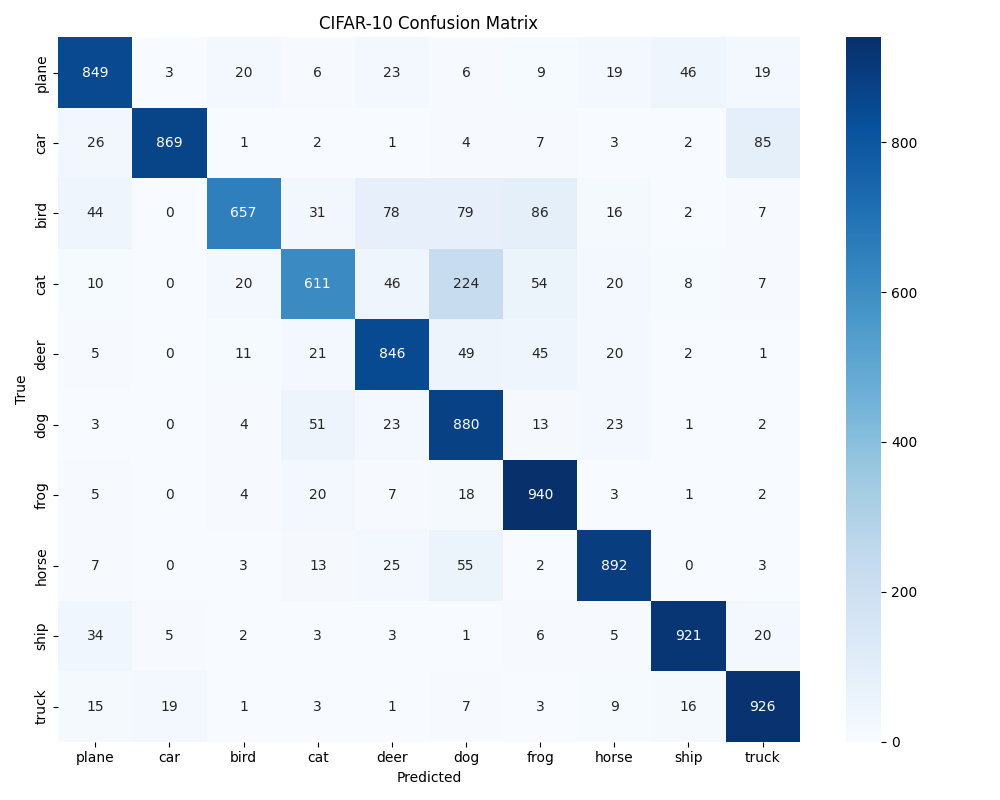
\includegraphics[width=0.47\textwidth]{images/task1_vgg11_confusion.png}
\hfill
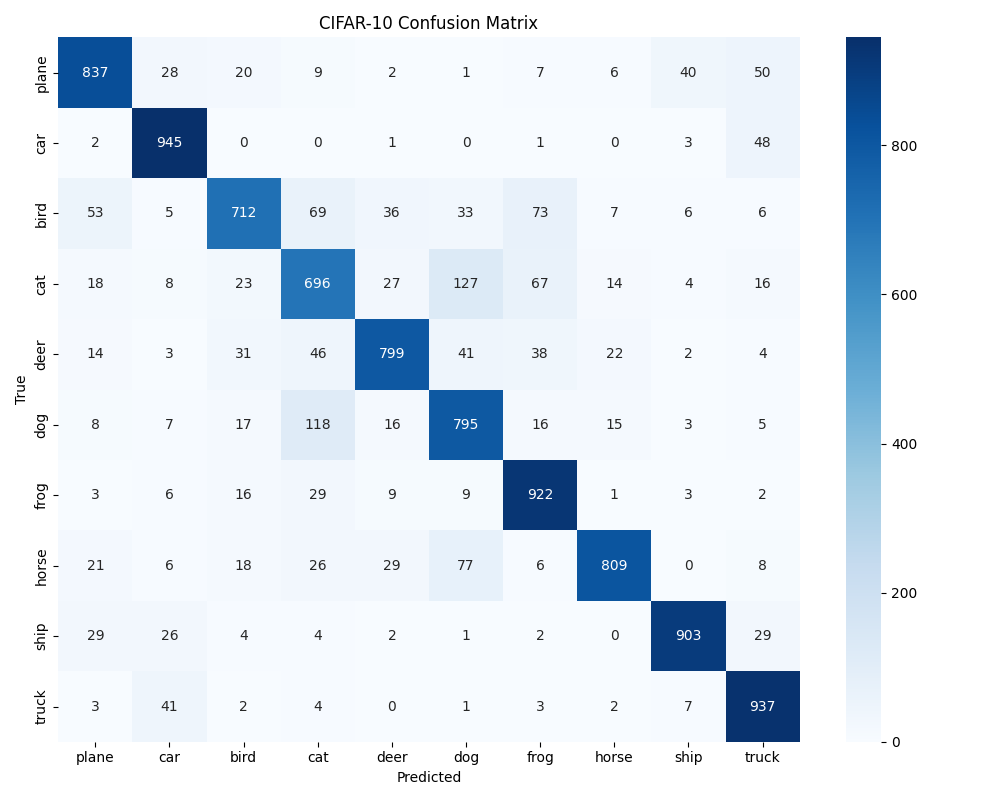
\includegraphics[width=0.47\textwidth]{images/task1_resnet20_confusion.png}
\caption{任务一混淆矩阵（左：VGG11，右：ResNet20）}
\label{fig:task1_cm}
\end{figure}

\subsection{任务二结果：ECG5000 多步预测对比}
根据实验统计结果，得到对比如表 \ref{tab:task2}。

\begin{table}[H]
\centering
\caption{任务二模型对比结果}
\label{tab:task2}
\begin{tabular}{lccc}
\toprule
模型 & 最优测试 MSE & 最终测试 MAE & 训练耗时（s） \\
\midrule
LSTM & 0.1535 & 0.2021 & 73.29 \\
GRU  & 0.1515 & 0.2036 & 43.32 \\
\bottomrule
\end{tabular}
\end{table}

结果分析：
\begin{itemize}
  \item 在 MSE 指标上，GRU 略优于 LSTM，说明其对整体平方误差控制稍好。
  \item 在 MAE 指标上，LSTM 略优于 GRU，二者差异很小。
  \item 训练耗时上，GRU 明显更快，参数更精简时具有效率优势。
\end{itemize}

\begin{figure}[H]
\centering
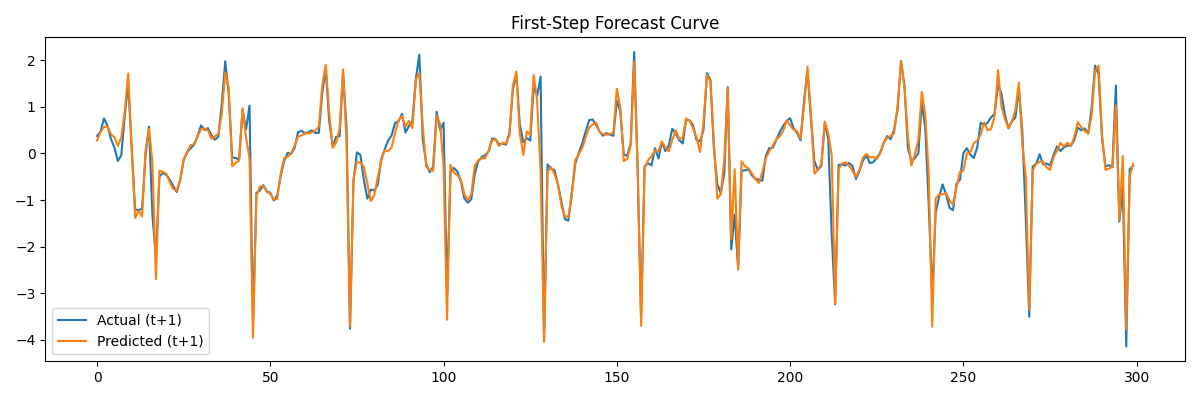
\includegraphics[width=0.47\textwidth]{images/task2_lstm_first_step.png}
\hfill
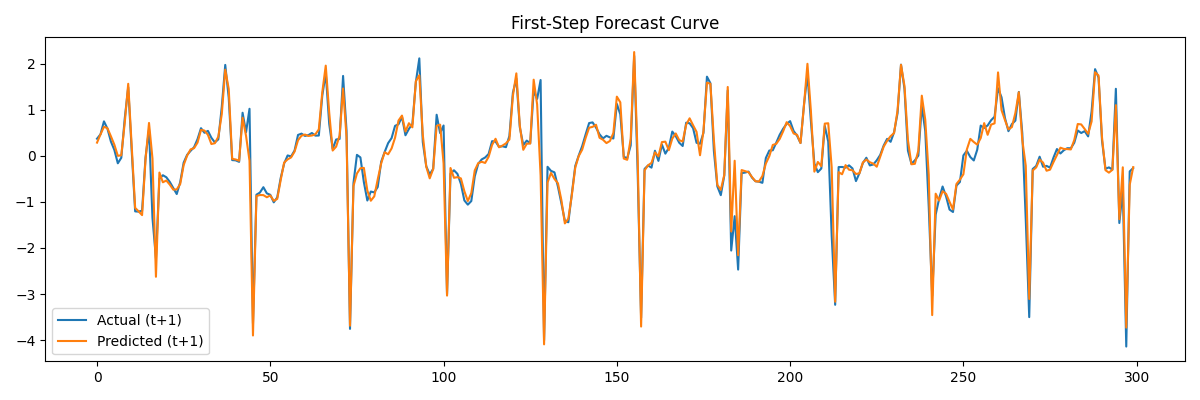
\includegraphics[width=0.47\textwidth]{images/task2_gru_first_step.png}
\caption{第一步预测曲线对比（左：LSTM，右：GRU）}
\label{fig:task2_curve}
\end{figure}

\begin{figure}[H]
\centering
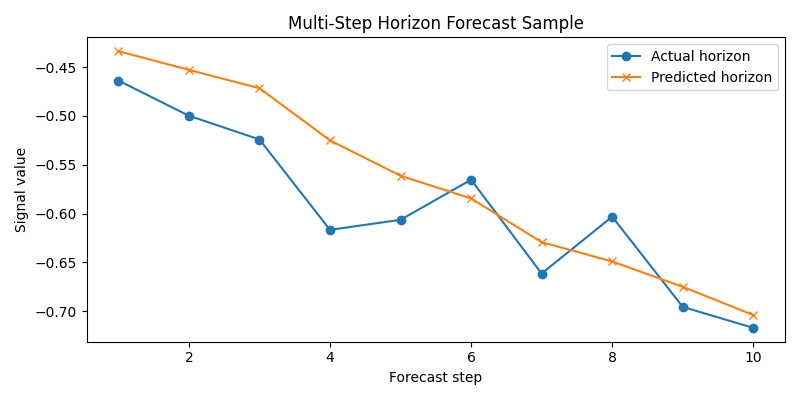
\includegraphics[width=0.47\textwidth]{images/task2_lstm_horizon.png}
\hfill
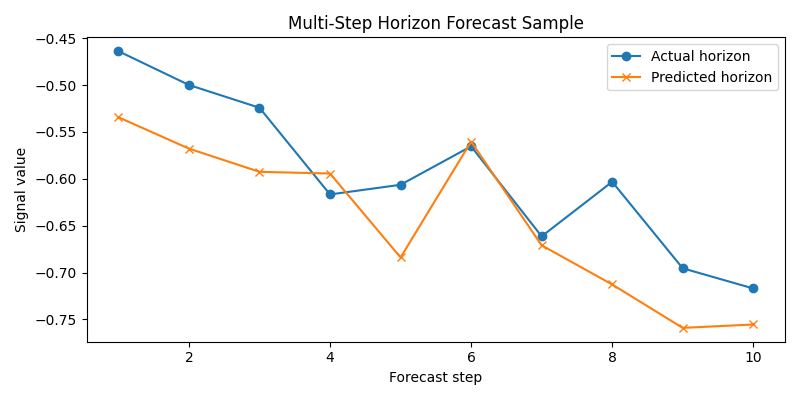
\includegraphics[width=0.47\textwidth]{images/task2_gru_horizon.png}
\caption{多步预测样本对比（左：LSTM，右：GRU）}
\label{fig:task2_horizon}
\end{figure}

\section{总结}
本实验完成了两类典型深度学习任务：
\begin{itemize}
  \item 图像分类任务中，VGG11 取得了更高的分类准确率，而 ResNet20 在训练速度与损失收敛上表现更均衡。
  \item 时序预测任务中，GRU 在 MSE 与训练效率上更有优势，LSTM 在 MAE 上略优，二者均能完成稳定的多步预测。
  \item 通过调整模型结构与训练超参数，可以在精度、误差与计算代价之间实现不同权衡。
\end{itemize}

\section*{附录：实验源代码与运行命令}
\subsection*{A.1 图像分类源码（task1\_cifar\_vgg\_resnet.py）}
\begin{lstlisting}
import argparse
import json
import random
import time
from pathlib import Path

import matplotlib.pyplot as plt
import numpy as np
import seaborn as sns
import torch
import torch.nn as nn
import torch.optim as optim
import torchvision
import torchvision.transforms as transforms
from sklearn.metrics import confusion_matrix
from torch.utils.data import DataLoader


def set_seed(seed: int) -> None:
  random.seed(seed)
  np.random.seed(seed)
  torch.manual_seed(seed)
  torch.cuda.manual_seed_all(seed)


class VGGClassifier(nn.Module):
  CFGS = {
    "vgg9": [64, "M", 128, "M", 256, 256, "M"],
    "vgg11": [64, "M", 128, "M", 256, 256, "M", 512, 512, "M"],
  }

  def __init__(self, variant: str = "vgg9", num_classes: int = 10):
    super().__init__()
    if variant not in self.CFGS:
      raise ValueError(f"Unsupported VGG variant: {variant}")
    self.features = self._make_layers(self.CFGS[variant])
    self.classifier = nn.Sequential(
      nn.Flatten(),
      nn.Linear(512, 256),
      nn.ReLU(inplace=True),
      nn.Dropout(0.4),
      nn.Linear(256, num_classes),
    )

  @staticmethod
  def _make_layers(cfg):
    layers = []
    in_ch = 3
    last_out_ch = 3
    for layer in cfg:
      if layer == "M":
        layers.append(nn.MaxPool2d(kernel_size=2, stride=2))
      else:
        layers.append(nn.Conv2d(in_ch, layer, kernel_size=3, padding=1, bias=False))
        layers.append(nn.BatchNorm2d(layer))
        layers.append(nn.ReLU(inplace=True))
        in_ch = layer
        last_out_ch = layer
    layers.append(nn.AdaptiveAvgPool2d((1, 1)))
    if last_out_ch < 512:
      layers.append(nn.Conv2d(last_out_ch, 512, kernel_size=1, bias=False))
      layers.append(nn.BatchNorm2d(512))
      layers.append(nn.ReLU(inplace=True))
    return nn.Sequential(*layers)

  def forward(self, x):
    x = self.features(x)
    return self.classifier(x)


class BasicBlock(nn.Module):
  expansion = 1

  def __init__(self, in_planes, planes, stride=1):
    super().__init__()
    self.conv1 = nn.Conv2d(in_planes, planes, kernel_size=3, stride=stride, padding=1, bias=False)
    self.bn1 = nn.BatchNorm2d(planes)
    self.conv2 = nn.Conv2d(planes, planes, kernel_size=3, stride=1, padding=1, bias=False)
    self.bn2 = nn.BatchNorm2d(planes)
    self.shortcut = nn.Sequential()
    if stride != 1 or in_planes != planes:
      self.shortcut = nn.Sequential(
        nn.Conv2d(in_planes, planes, kernel_size=1, stride=stride, bias=False),
        nn.BatchNorm2d(planes),
      )

  def forward(self, x):
    out = torch.relu(self.bn1(self.conv1(x)))
    out = self.bn2(self.conv2(out))
    out += self.shortcut(x)
    return torch.relu(out)


class ResNetCifar(nn.Module):
  def __init__(self, depth=20, num_classes=10):
    super().__init__()
    if (depth - 2) % 6 != 0:
      raise ValueError("ResNet depth must satisfy 6n+2 for CIFAR (e.g., 14, 20, 32)")
    n = (depth - 2) // 6
    self.in_planes = 16

    self.conv1 = nn.Conv2d(3, 16, kernel_size=3, stride=1, padding=1, bias=False)
    self.bn1 = nn.BatchNorm2d(16)
    self.layer1 = self._make_layer(16, n, stride=1)
    self.layer2 = self._make_layer(32, n, stride=2)
    self.layer3 = self._make_layer(64, n, stride=2)
    self.avgpool = nn.AdaptiveAvgPool2d((1, 1))
    self.fc = nn.Linear(64, num_classes)

  def _make_layer(self, planes, blocks, stride):
    layers = [BasicBlock(self.in_planes, planes, stride)]
    self.in_planes = planes
    for _ in range(1, blocks):
      layers.append(BasicBlock(self.in_planes, planes, stride=1))
    return nn.Sequential(*layers)

  def forward(self, x):
    out = torch.relu(self.bn1(self.conv1(x)))
    out = self.layer1(out)
    out = self.layer2(out)
    out = self.layer3(out)
    out = self.avgpool(out)
    out = torch.flatten(out, 1)
    return self.fc(out)


def get_dataloaders(data_root: Path, batch_size: int, num_workers: int):
  transform_train = transforms.Compose(
    [
      transforms.RandomCrop(32, padding=4),
      transforms.RandomHorizontalFlip(),
      transforms.ToTensor(),
      transforms.Normalize((0.4914, 0.4822, 0.4465), (0.2023, 0.1994, 0.2010)),
    ]
  )
  transform_test = transforms.Compose(
    [
      transforms.ToTensor(),
      transforms.Normalize((0.4914, 0.4822, 0.4465), (0.2023, 0.1994, 0.2010)),
    ]
  )

  train_set = torchvision.datasets.CIFAR10(root=str(data_root), train=True, download=True, transform=transform_train)
  test_set = torchvision.datasets.CIFAR10(root=str(data_root), train=False, download=True, transform=transform_test)

  train_loader = DataLoader(train_set, batch_size=batch_size, shuffle=True, num_workers=num_workers)
  test_loader = DataLoader(test_set, batch_size=batch_size, shuffle=False, num_workers=num_workers)
  return train_loader, test_loader


def choose_optimizer(name: str, model: nn.Module, lr: float, weight_decay: float):
  if name == "adam":
    return optim.Adam(model.parameters(), lr=lr, weight_decay=weight_decay)
  if name == "sgd":
    return optim.SGD(model.parameters(), lr=lr, momentum=0.9, weight_decay=weight_decay)
  raise ValueError(f"Unsupported optimizer: {name}")


def run_epoch(model, loader, criterion, optimizer, device):
  model.train()
  total_loss = 0.0
  total_correct = 0
  total = 0

  for images, labels in loader:
    images = images.to(device)
    labels = labels.to(device)
    optimizer.zero_grad()
    logits = model(images)
    loss = criterion(logits, labels)
    loss.backward()
    optimizer.step()

    total_loss += loss.item() * labels.size(0)
    preds = torch.argmax(logits, dim=1)
    total_correct += (preds == labels).sum().item()
    total += labels.size(0)

  return total_loss / total, total_correct / total


def evaluate(model, loader, criterion, device, collect_predictions=False):
  model.eval()
  total_loss = 0.0
  total_correct = 0
  total = 0
  all_labels = []
  all_preds = []

  with torch.no_grad():
    for images, labels in loader:
      images = images.to(device)
      labels = labels.to(device)
      logits = model(images)
      loss = criterion(logits, labels)

      total_loss += loss.item() * labels.size(0)
      preds = torch.argmax(logits, dim=1)
      total_correct += (preds == labels).sum().item()
      total += labels.size(0)

      if collect_predictions:
        all_labels.extend(labels.cpu().numpy().tolist())
        all_preds.extend(preds.cpu().numpy().tolist())

  result = {
    "loss": total_loss / total,
    "acc": total_correct / total,
  }
  if collect_predictions:
    result["labels"] = all_labels
    result["preds"] = all_preds
  return result


def save_confusion_matrix(labels, preds, classes, out_path: Path):
  cm = confusion_matrix(labels, preds)
  plt.figure(figsize=(10, 8))
  sns.heatmap(cm, annot=True, fmt="d", cmap="Blues", xticklabels=classes, yticklabels=classes)
  plt.xlabel("Predicted")
  plt.ylabel("True")
  plt.title("CIFAR-10 Confusion Matrix")
  plt.tight_layout()
  plt.savefig(out_path)
  plt.close()


def train_and_evaluate(model_name: str, args, train_loader, test_loader, device, classes, output_root: Path):
  if model_name == "vgg":
    model = VGGClassifier(variant=args.vgg_variant).to(device)
    model_tag = args.vgg_variant
  elif model_name == "resnet":
    model = ResNetCifar(depth=args.resnet_depth).to(device)
    model_tag = f"resnet{args.resnet_depth}"
  else:
    raise ValueError(f"Unsupported model name: {model_name}")

  run_dir = output_root / model_tag
  run_dir.mkdir(parents=True, exist_ok=True)

  criterion = nn.CrossEntropyLoss()
  optimizer = choose_optimizer(args.optimizer, model, args.lr, args.weight_decay)

  best_acc = 0.0
  history = []
  best_path = run_dir / "best_model.pth"

  start = time.time()
  for epoch in range(1, args.epochs + 1):
    train_loss, train_acc = run_epoch(model, train_loader, criterion, optimizer, device)
    val_result = evaluate(model, test_loader, criterion, device)
    epoch_result = {
      "epoch": epoch,
      "train_loss": train_loss,
      "train_acc": train_acc,
      "test_loss": val_result["loss"],
      "test_acc": val_result["acc"],
    }
    history.append(epoch_result)

    if val_result["acc"] > best_acc:
      best_acc = val_result["acc"]
      torch.save(model.state_dict(), best_path)

    print(
      f"[{model_tag}] Epoch {epoch:03d}/{args.epochs:03d} | "
      f"Train Acc {train_acc * 100:.2f}% | Test Acc {val_result['acc'] * 100:.2f}%"
    )

  model.load_state_dict(torch.load(best_path, map_location=device))
  final_result = evaluate(model, test_loader, criterion, device, collect_predictions=True)
  save_confusion_matrix(
    final_result["labels"],
    final_result["preds"],
    classes,
    run_dir / "confusion_matrix.png",
  )

  summary = {
    "model": model_tag,
    "epochs": args.epochs,
    "optimizer": args.optimizer,
    "lr": args.lr,
    "batch_size": args.batch_size,
    "weight_decay": args.weight_decay,
    "best_test_acc": best_acc,
    "final_test_acc": final_result["acc"],
    "final_test_loss": final_result["loss"],
    "train_seconds": time.time() - start,
    "history": history,
  }

  with (run_dir / "metrics.json").open("w", encoding="utf-8") as f:
    json.dump(summary, f, indent=2)

  return summary


def parse_args():
  parser = argparse.ArgumentParser(description="Task 1: CIFAR-10 classification with VGG/ResNet")
  parser.add_argument("--model", choices=["vgg", "resnet", "both"], default="both")
  parser.add_argument("--vgg_variant", choices=["vgg9", "vgg11"], default="vgg11")
  parser.add_argument("--resnet_depth", type=int, default=20, help="Valid examples: 14, 20, 32")
  parser.add_argument("--epochs", type=int, default=20)
  parser.add_argument("--batch_size", type=int, default=128)
  parser.add_argument("--optimizer", choices=["adam", "sgd"], default="adam")
  parser.add_argument("--lr", type=float, default=1e-3)
  parser.add_argument("--weight_decay", type=float, default=5e-4)
  parser.add_argument("--num_workers", type=int, default=2)
  parser.add_argument("--seed", type=int, default=42)
  parser.add_argument("--data_root", type=str, default="./cifar-10-batches-py")
  parser.add_argument("--output_dir", type=str, default="./outputs/task1")
  return parser.parse_args()


def main():
  args = parse_args()
  set_seed(args.seed)

  device = torch.device("cuda" if torch.cuda.is_available() else "cpu")
  classes = ["plane", "car", "bird", "cat", "deer", "dog", "frog", "horse", "ship", "truck"]

  data_root = Path(args.data_root)
  output_root = Path(args.output_dir)
  output_root.mkdir(parents=True, exist_ok=True)

  train_loader, test_loader = get_dataloaders(data_root, args.batch_size, args.num_workers)

  models_to_run = [args.model] if args.model != "both" else ["vgg", "resnet"]
  summaries = []
  for model_name in models_to_run:
    summaries.append(train_and_evaluate(model_name, args, train_loader, test_loader, device, classes, output_root))

  if len(summaries) == 2:
    comparison = {
      "task": "cifar10_vgg_resnet_comparison",
      "vgg": summaries[0],
      "resnet": summaries[1],
      "better_model": summaries[0]["model"] if summaries[0]["final_test_acc"] >= summaries[1]["final_test_acc"] else summaries[1]["model"],
    }
    with (output_root / "comparison.json").open("w", encoding="utf-8") as f:
      json.dump(comparison, f, indent=2)
    print(f"Comparison written to {output_root / 'comparison.json'}")


if __name__ == "__main__":
  main()
\end{lstlisting}

\subsection*{A.2 时序预测源码（task2\_ecg\_lstm\_gru.py）}
\begin{lstlisting}
import argparse
import json
import random
import time
from pathlib import Path

import matplotlib.pyplot as plt
import numpy as np
import pandas as pd
import torch
import torch.nn as nn
import torch.optim as optim
from torch.utils.data import DataLoader, Dataset


class SequenceDataset(Dataset):
  def __init__(self, x, y):
    self.x = torch.from_numpy(x).float()
    self.y = torch.from_numpy(y).float()

  def __len__(self):
    return len(self.x)

  def __getitem__(self, idx):
    return self.x[idx], self.y[idx]


def set_seed(seed: int) -> None:
  random.seed(seed)
  np.random.seed(seed)
  torch.manual_seed(seed)
  torch.cuda.manual_seed_all(seed)


def load_ecg5000_series(train_path: Path, test_path: Path):
  train_df = pd.read_csv(train_path, sep=r"\s+", header=None)
  test_df = pd.read_csv(test_path, sep=r"\s+", header=None)

  train_features = train_df.iloc[:, 1:].to_numpy(dtype=np.float32)
  test_features = test_df.iloc[:, 1:].to_numpy(dtype=np.float32)

  train_series = train_features.reshape(-1)
  test_series = test_features.reshape(-1)

  mean = train_series.mean()
  std = train_series.std() + 1e-8
  train_series = (train_series - mean) / std
  test_series = (test_series - mean) / std

  return train_series, test_series, mean, std


def make_windows(series: np.ndarray, input_len: int, pred_len: int, stride: int):
  x, y = [], []
  end = len(series) - input_len - pred_len + 1
  for i in range(0, end, stride):
    x.append(series[i : i + input_len])
    y.append(series[i + input_len : i + input_len + pred_len])
  x = np.asarray(x, dtype=np.float32)[..., np.newaxis]
  y = np.asarray(y, dtype=np.float32)
  return x, y


class RNNForecaster(nn.Module):
  def __init__(self, model_type: str, hidden_size: int, num_layers: int, dropout: float, pred_len: int):
    super().__init__()
    rnn_cls = nn.LSTM if model_type == "lstm" else nn.GRU
    effective_dropout = dropout if num_layers > 1 else 0.0
    self.rnn = rnn_cls(
      input_size=1,
      hidden_size=hidden_size,
      num_layers=num_layers,
      batch_first=True,
      dropout=effective_dropout,
    )
    self.fc = nn.Linear(hidden_size, pred_len)

  def forward(self, x):
    out, _ = self.rnn(x)
    return self.fc(out[:, -1, :])


def choose_optimizer(name: str, model: nn.Module, lr: float, weight_decay: float):
  if name == "adam":
    return optim.Adam(model.parameters(), lr=lr, weight_decay=weight_decay)
  if name == "sgd":
    return optim.SGD(model.parameters(), lr=lr, momentum=0.9, weight_decay=weight_decay)
  raise ValueError(f"Unsupported optimizer: {name}")


def train_one_epoch(model, loader, criterion, optimizer, device):
  model.train()
  total_loss = 0.0
  total = 0
  for x_batch, y_batch in loader:
    x_batch = x_batch.to(device)
    y_batch = y_batch.to(device)

    optimizer.zero_grad()
    pred = model(x_batch)
    loss = criterion(pred, y_batch)
    loss.backward()
    optimizer.step()

    total_loss += loss.item() * y_batch.size(0)
    total += y_batch.size(0)
  return total_loss / total


def evaluate(model, loader, criterion, device):
  model.eval()
  total_loss = 0.0
  total = 0
  preds = []
  trues = []

  with torch.no_grad():
    for x_batch, y_batch in loader:
      x_batch = x_batch.to(device)
      y_batch = y_batch.to(device)
      pred = model(x_batch)
      loss = criterion(pred, y_batch)

      total_loss += loss.item() * y_batch.size(0)
      total += y_batch.size(0)
      preds.append(pred.cpu().numpy())
      trues.append(y_batch.cpu().numpy())

  preds = np.concatenate(preds, axis=0)
  trues = np.concatenate(trues, axis=0)
  mae = np.mean(np.abs(preds - trues))
  return float(total_loss / total), float(mae), trues, preds


def save_plots(trues, preds, mean, std, run_dir: Path, plot_points: int):
  trues_denorm = trues * std + mean
  preds_denorm = preds * std + mean

  first_step_true = trues_denorm[:, 0]
  first_step_pred = preds_denorm[:, 0]
  n = min(plot_points, len(first_step_true))

  plt.figure(figsize=(12, 4))
  plt.plot(first_step_true[:n], label="Actual (t+1)")
  plt.plot(first_step_pred[:n], label="Predicted (t+1)")
  plt.title("First-Step Forecast Curve")
  plt.legend()
  plt.tight_layout()
  plt.savefig(run_dir / "first_step_curve.png")
  plt.close()

  sample_idx = min(len(trues_denorm) - 1, 20)
  horizon_true = trues_denorm[sample_idx]
  horizon_pred = preds_denorm[sample_idx]
  horizon = np.arange(1, len(horizon_true) + 1)

  plt.figure(figsize=(8, 4))
  plt.plot(horizon, horizon_true, marker="o", label="Actual horizon")
  plt.plot(horizon, horizon_pred, marker="x", label="Predicted horizon")
  plt.title("Multi-Step Horizon Forecast Sample")
  plt.xlabel("Forecast step")
  plt.ylabel("Signal value")
  plt.legend()
  plt.tight_layout()
  plt.savefig(run_dir / "horizon_sample.png")
  plt.close()


def run_single_model(model_name, args, train_loader, test_loader, mean, std, device, output_root: Path):
  run_dir = output_root / model_name
  run_dir.mkdir(parents=True, exist_ok=True)

  model = RNNForecaster(
    model_type=model_name,
    hidden_size=args.hidden_size,
    num_layers=args.num_layers,
    dropout=args.dropout,
    pred_len=args.pred_len,
  ).to(device)

  criterion = nn.MSELoss()
  optimizer = choose_optimizer(args.optimizer, model, args.lr, args.weight_decay)

  best_mse = float("inf")
  history = []
  best_path = run_dir / "best_model.pth"

  start = time.time()
  for epoch in range(1, args.epochs + 1):
    train_loss = train_one_epoch(model, train_loader, criterion, optimizer, device)
    test_mse, test_mae, _, _ = evaluate(model, test_loader, criterion, device)

    history.append({
      "epoch": epoch,
      "train_mse": float(train_loss),
      "test_mse": float(test_mse),
      "test_mae": float(test_mae),
    })

    if test_mse < best_mse:
      best_mse = test_mse
      torch.save(model.state_dict(), best_path)

    print(
      f"[{model_name}] Epoch {epoch:03d}/{args.epochs:03d} | "
      f"Train MSE {train_loss:.6f} | Test MSE {test_mse:.6f} | Test MAE {test_mae:.6f}"
    )

  model.load_state_dict(torch.load(best_path, map_location=device))
  final_mse, final_mae, trues, preds = evaluate(model, test_loader, criterion, device)
  save_plots(trues, preds, mean, std, run_dir, args.plot_points)

  metrics = {
    "model": model_name,
    "input_len": args.input_len,
    "pred_len": args.pred_len,
    "epochs": args.epochs,
    "optimizer": args.optimizer,
    "lr": args.lr,
    "batch_size": args.batch_size,
    "best_test_mse": float(best_mse),
    "final_test_mse": float(final_mse),
    "final_test_mae": float(final_mae),
    "train_seconds": float(time.time() - start),
    "history": history,
  }

  with (run_dir / "metrics.json").open("w", encoding="utf-8") as f:
    json.dump(metrics, f, indent=2)

  return metrics


def parse_args():
  parser = argparse.ArgumentParser(description="Task 2: ECG5000 multi-step forecasting with LSTM/GRU")
  parser.add_argument("--model", choices=["lstm", "gru", "both"], default="both")
  parser.add_argument("--train_path", type=str, default="./ECG5000/ECG5000_TRAIN.tsv")
  parser.add_argument("--test_path", type=str, default="./ECG5000/ECG5000_TEST.tsv")
  parser.add_argument("--input_len", type=int, default=60, help="Input window size m")
  parser.add_argument("--pred_len", type=int, default=10, help="Prediction horizon p (1=single-step)")
  parser.add_argument("--stride", type=int, default=5, help="Window sampling stride")
  parser.add_argument("--hidden_size", type=int, default=128)
  parser.add_argument("--num_layers", type=int, default=2)
  parser.add_argument("--dropout", type=float, default=0.2)
  parser.add_argument("--epochs", type=int, default=30)
  parser.add_argument("--batch_size", type=int, default=128)
  parser.add_argument("--optimizer", choices=["adam", "sgd"], default="adam")
  parser.add_argument("--lr", type=float, default=1e-3)
  parser.add_argument("--weight_decay", type=float, default=0.0)
  parser.add_argument("--num_workers", type=int, default=0)
  parser.add_argument("--plot_points", type=int, default=300)
  parser.add_argument("--output_dir", type=str, default="./outputs/task2")
  parser.add_argument("--seed", type=int, default=42)
  return parser.parse_args()


def main():
  args = parse_args()
  set_seed(args.seed)
  device = torch.device("cuda" if torch.cuda.is_available() else "cpu")

  train_series, test_series, mean, std = load_ecg5000_series(Path(args.train_path), Path(args.test_path))
  x_train, y_train = make_windows(train_series, args.input_len, args.pred_len, args.stride)
  x_test, y_test = make_windows(test_series, args.input_len, args.pred_len, args.stride)

  train_dataset = SequenceDataset(x_train, y_train)
  test_dataset = SequenceDataset(x_test, y_test)

  train_loader = DataLoader(train_dataset, batch_size=args.batch_size, shuffle=True, num_workers=args.num_workers)
  test_loader = DataLoader(test_dataset, batch_size=args.batch_size, shuffle=False, num_workers=args.num_workers)

  output_root = Path(args.output_dir)
  output_root.mkdir(parents=True, exist_ok=True)

  models_to_run = [args.model] if args.model != "both" else ["lstm", "gru"]
  summaries = []
  for model_name in models_to_run:
    summaries.append(run_single_model(model_name, args, train_loader, test_loader, mean, std, device, output_root))

  if len(summaries) == 2:
    comparison = {
      "task": "ecg5000_lstm_gru_multistep_comparison",
      "lstm": summaries[0],
      "gru": summaries[1],
      "better_model": summaries[0]["model"] if summaries[0]["final_test_mse"] <= summaries[1]["final_test_mse"] else summaries[1]["model"],
    }
    with (output_root / "comparison.json").open("w", encoding="utf-8") as f:
      json.dump(comparison, f, indent=2)
    print(f"Comparison written to {output_root / 'comparison.json'}")


if __name__ == "__main__":
  main()
\end{lstlisting}

\subsection*{A.3 复现实验命令}
\begin{verbatim}
# 任务一：VGG + ResNet 分类对比
python task1_cifar_vgg_resnet.py --model both --epochs 20 \
  --batch_size 128 --optimizer adam --lr 0.001 \
  --vgg_variant vgg11 --resnet_depth 20

# 任务二：LSTM + GRU 多步预测对比
python task2_ecg_lstm_gru.py --model both --input_len 60 --pred_len 10 \
  --epochs 30 --batch_size 128 --optimizer adam --lr 0.001
\end{verbatim}

\end{document}
